\chapter{Introdução} 
	\label{ch:introducao}

Veículos automotores estão presente no nosso dia a dia há mais de 100 anos \cite{fordt} e nunca param de evoluir. Tais  máquinas que por anos eram peças de engenharia mecânica tem recebido uma mudança de paradigma. Os carros tem acumulado eletrônica para desempenhar funções simples e complexas que algumas décadas atrás eram impossíveis. Sensores, atuadores e centrais eletrônicas de processamento podem ser usados para auxílio na segurança, com detecção de faixas de pista, auxílio em frenagem antecipada e controle de estabilidade \cite{racecarInstrumentationFor2012}, em aplicações de conforto com sensores de temperatura do ambiente para controlar aparelhos condicionadores de ar digital e também em aplicações de performance, onde os sistemas atuam para entregar uma melhora de desempenho do carro de acordo com sua situação em que o mesmo se encontra.

Ainda na área de performance, área de telemetria, aquisição de dados e tratamento de dados de um veículo é usada de forma extensiva em competições automobilísticas no qual a amostragem em tempo real é necessária para centenas de sensores que permitem aos engenheiros manterem o rastreamento da performance do \textit{powertrain}, parâmetros de dirigibilidade como configurações de suspensão e temperatura dos pneus \cite{designAndImplementation2015}. Estes dados são fundamentais para que os engenheiros e pilotos consigam acertar o carro a fim de obter tempo de voltas mais rápidos, além de melhor manutenção do carro de forma geral.

Dentro deste contexto, a equipe escolar de automobilismo Velociraptor\footnote{https://www.facebook.com/velociraptor.baja/} foi procurada para realização de um projeto que envolvesse automobilismo e ciência da computação. Depois de diversas reuniões com a equipe foi encontrada uma área em comum, a aquisição de dados e telemetria do veículo da categoria baja SAE codinome fênix, que pode ser visto na Figura \ref{fig:baja}. A ideia inicial era a criação de um sistema completo de telemetria veicular para um veículo \textit{off-road}, desde a criação de um sistema de controle \textit{on-board} (ou SCOB) que consiste em uma unidade de processamento para dados recebidos de sensores espalhados pelo carro com um microcontrolador, até um \textit{software} de tratamento dos dados recebidos via telemetria. Esta ideia foi modificada com o tempo e visto que o escopo de trabalho seria muito abrangente e o período de dois semestres não seria suficiente.    

\begin{figure}[!htb]
	\centering
		\caption{Veículo fênix da equipe baja Velociraptor.}
		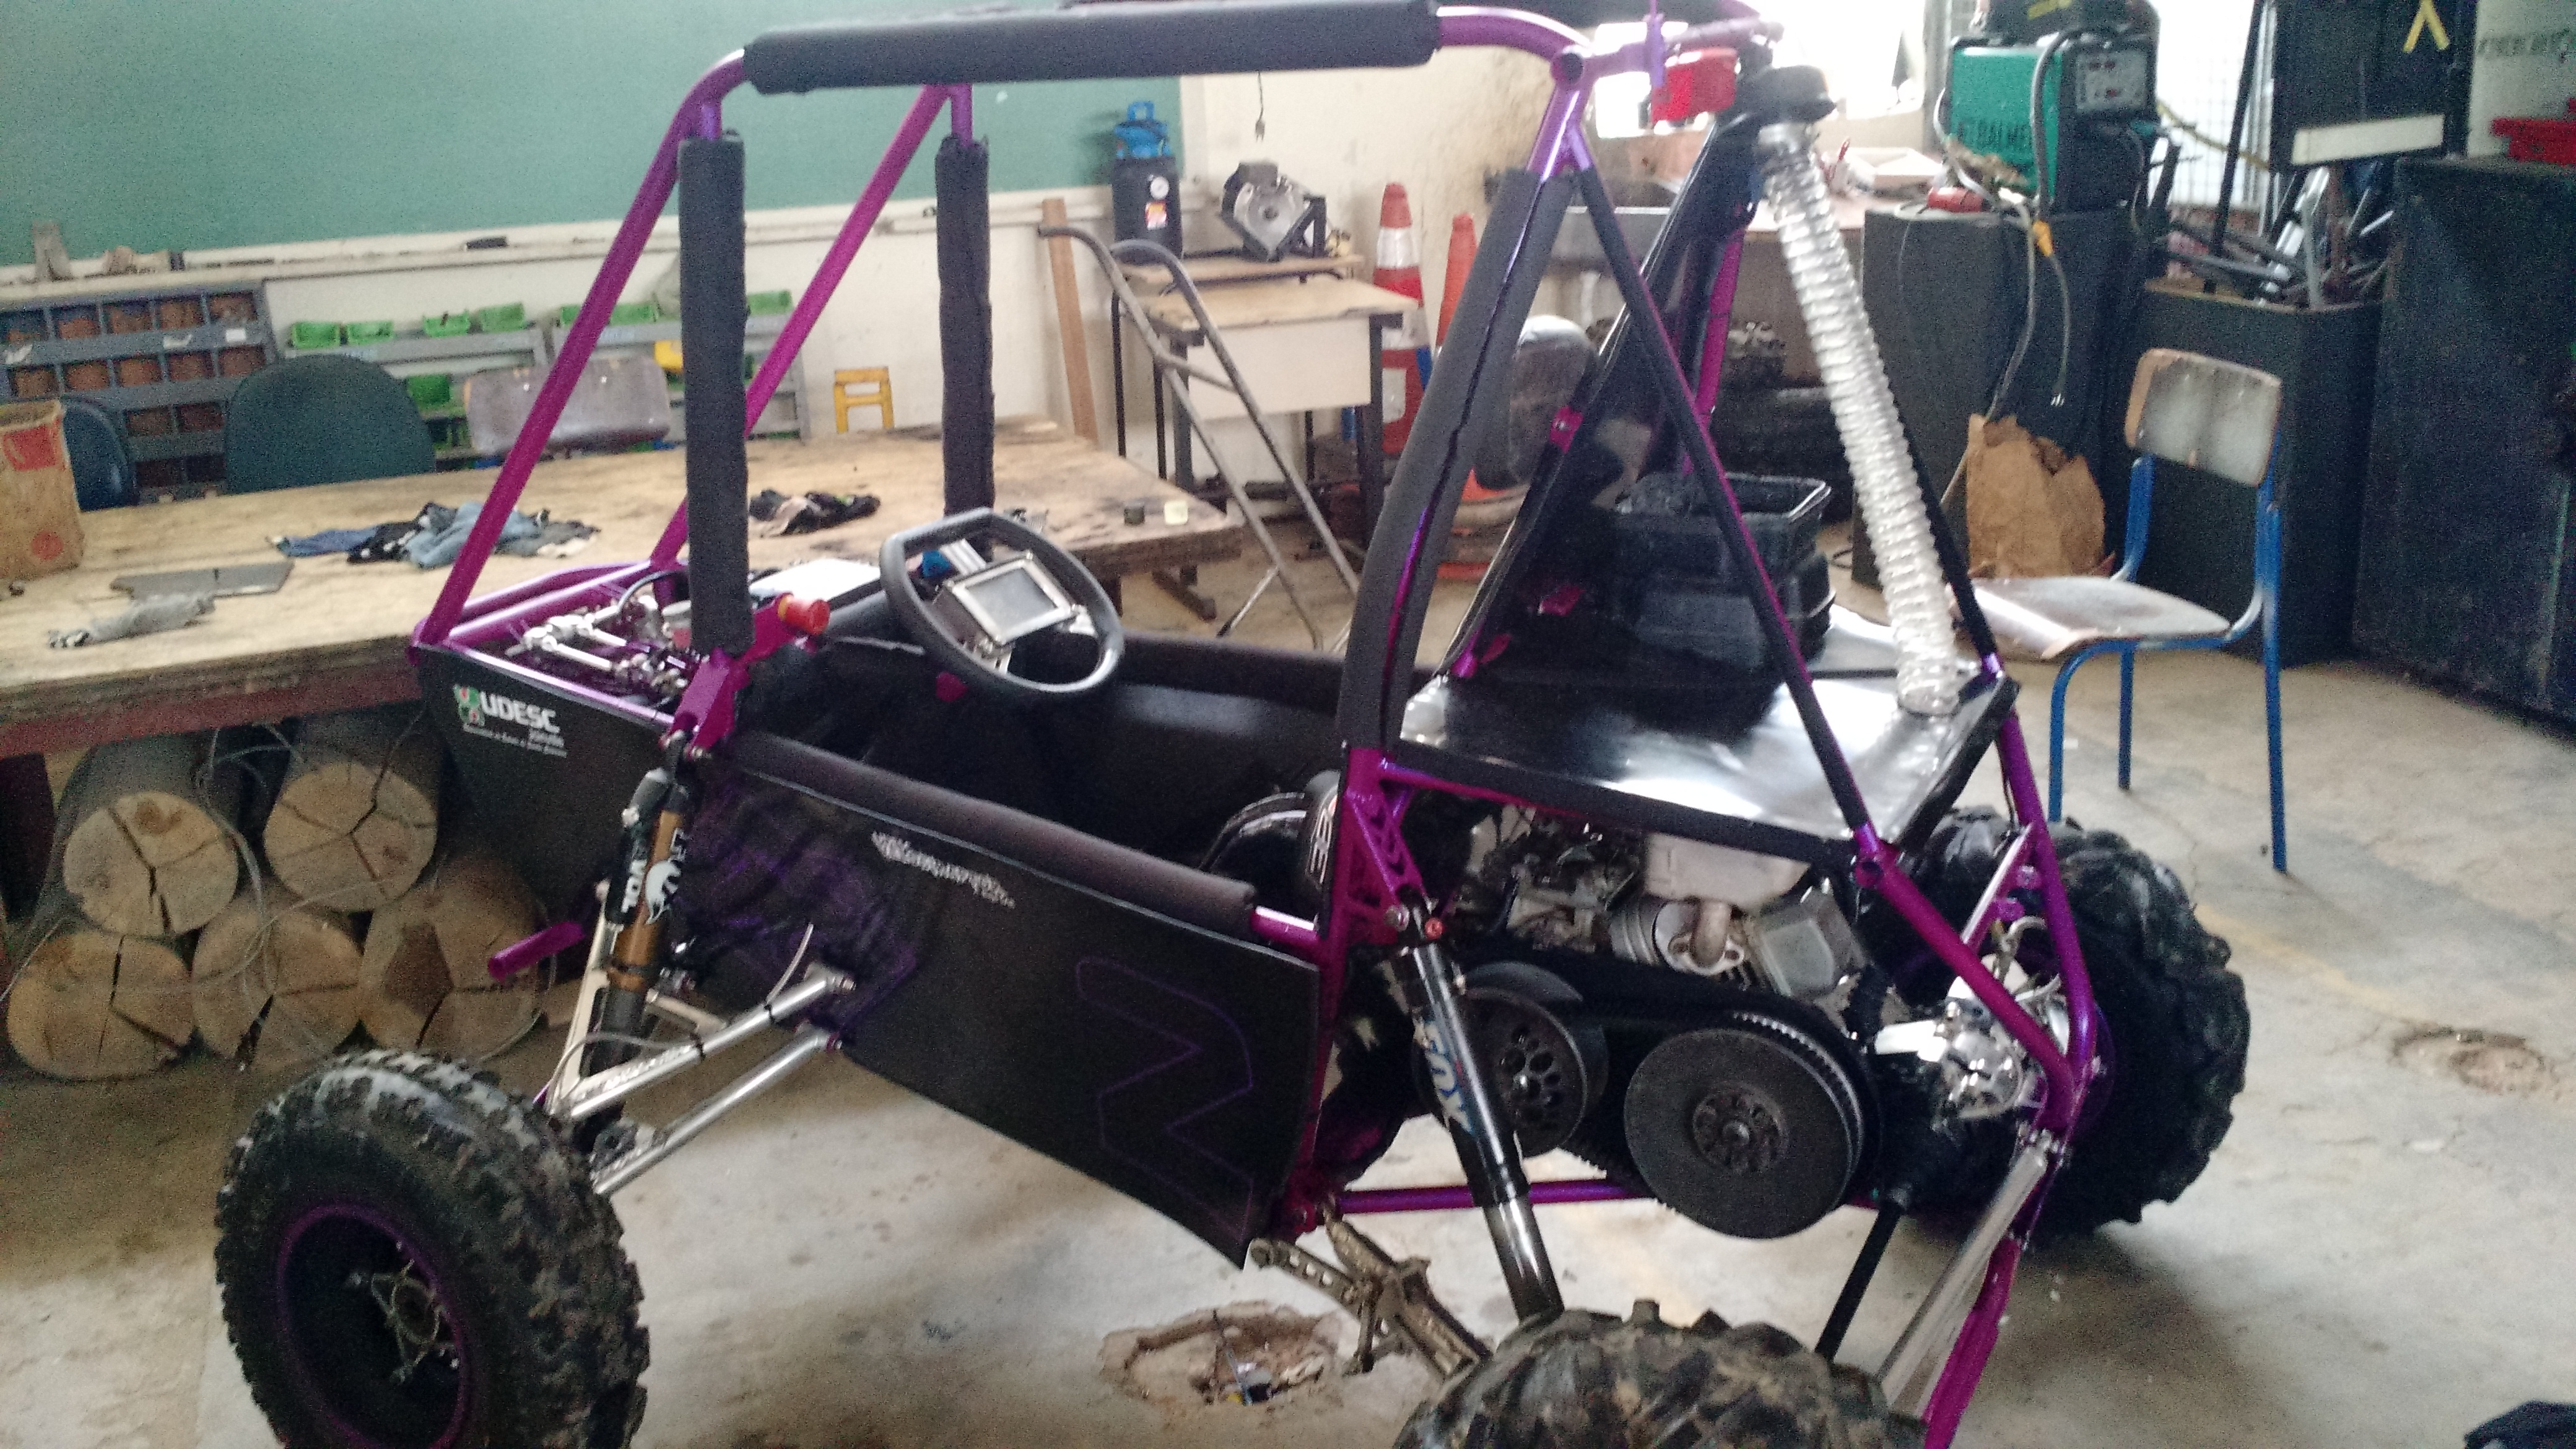
\includegraphics[scale=0.1]{baja} 
		\caption*{Fonte: Autor.}
		\label{fig:baja}
\end{figure} 

Uma nova proposta então foi realizada, a criação de um \textit{software} de tratamento dos dados recebidos do SCOB por meio de um \textit{Secure Digital Card}, ou como é normalmente conhecido cartão SD. Contudo, durante reuniões do projeto do sub-sistema de eletrônica veicular do Velociraptor, foi adicionado ao escopo de projeto o uso de telemetria para recepção dos dados. Tendo esta oportunidade em mente uma nova proposta é então concebida para a segunda parte deste trabalho na qual todas as características anteriormente requisitadas se mantem, exceto pelo uso do cartão SD como meio principal de envio e recepção dos dados. 
%Nesta nova proposta, o escopo de projeto é mais consistente com a linha de aprendizado do curso de ciências da computação, mais realista em relação ao tempo de execução do projeto e mais coerente com o que a equipe Velociraptor espera deste projeto conjunto. 
A equipe deseja obter melhores informações sobre o veículo de forma intuitiva com visualização dos dados com gráficos e separação das informações por setores automotivos, de forma simplificada com a utilização de um único programa para visualização das informações, com um programa feito de forma modular, ou seja, que esteja preparado para receber atualizações futuras de componentes e tecnologias e com armazenamento para melhor confiabilidade e comparações de informações de diversas provas de teste.   

Inicialmente alguns problemas encontrados no cenário de veículos \textit{off-road} podem ser analisados. Em \citeonline{projetoMiniBaja2006} alguns avisos sobre problemas que são comumente encontrados em situações de extremo esforço para o conjunto mecânico e eletrônico, como em uma prova de enduro do baja SAE. Estes problemas devem ser levados em consideração na hora de montagem do sistema de aquisição de dados e também do \textit{software} de tratamento de dados. Os problemas encontrados são:

\begin{itemize}
	\item  Interferência eletro-magnética: Os picos de tensão produzidos pela centelha da vela podem interferir no microcontrolador se o mesmo não for bem isolado; 
	\item Temperatura do \textit{cockpit}: Depende muito da hora de realização do enduro e local, mas em regiões mais quentes como no nordeste e em horários como 12 e 14 horas, a temperatura interna do \textit{cockpit} pode ficar muito elevada e esta pode comprometer qualquer circuito eletrônico que seja sensível a calor e não esteja protegido; 
	\item Vibração: Pela natureza de uma prova \textit{off-road}, existe muita vibração. Este problema pode acarretar em mal contato entre circuitos e placas;
	\item Lama e água: Devido ao contexto do projeto \textit{off-road} existe muitos obstáculos com lama e água no percurso dos testes e estes dois elementos podem danificar as placas eletrônicas.
\end{itemize}

Foram então levantados junto com a grupo Velociraptor vários componentes que a equipe deseja monitorar. Alguns destes componentes já estão instalados no veículo e fazem parte dos requisitos do projeto, na parte de grandezas que devem ser monitoradas. Os seguintes itens foram levantados: 

\begin{itemize}
	\item Frequência de rotação do motor;
	\item Velocidade do veículo;
	\item Nível do combustível;
	\item Relação de transmissão;
	\item Temperatura do câmbio CVT;
	\item Rolagem da carroceria;
	\item Deslocamento do amortecedor;
	\item Deslocamento da suspensão;
	\item Temperatura do disco de freio;
\end{itemize}

Enquanto algumas grandezas não fazem parte do escopo inicial deste projeto, as que fazem são analisadas na fundamentação teórica. As grandezas serão recebidas no computador dos boxes a partir do SCOB e transmitidas via protocolo ZigBee para a plataforma de tratamento de dados. Com este trabalho é esperado que a equipe consiga manter informações valiosas sobre o veículo que não poderiam ser obtidas de outra forma. A utilização de um \textit{software} de monitoramento é um passo importante para atingir um melhor desempenho na hora da manutenção, construção e realização de novos projetos para os veículos focados em automobilismo.   

\section{Estrutura do trabalho}

O trabalho a seguir é estruturado da seguinte forma. O Capítulo \ref{ch:fundamentacao} traz uma revisão de conceitos que serão utilizados no trabalho. Os conceitos abordados incluem o funcionamento e organização da prova da categoria baja SAE, com alguns detalhes das regras impostas para produção do veículo \textit{off-road}, uma revisão de vários sensores utilizados para a captura de grandezas do veículo, um estudo sobre microcontroladores para adequação de novas tecnologias sobre o sistema embarcado do veículo, uma análise sobre o protocolo de transmissão de dados sem fio e por fim um estudo sobre os objetivos dos sistemas de tratamento e aquisição de dados. No Capítulo \ref{ch:trabalhos} é realizado um estudo sobre o que existe de estado da arte em aquisição de dados na área automotiva, com foco em trabalhos voltados para o automobilismo. No Capítulo \ref{ch:proposta} é apresentada a proposta de trabalho, junto com os objetivos específicos que devem ser alcançados no percurso de sua realização. No Capítulo \ref{ch:desenvolvimento} é discutido sobre o desenvolvimento do sistema de tratamento e de aquisição de dados. No Capítulo \ref{ch:testes} são discutidos os testes realizados no sistema para validação dos resultados. Por último no Capítulo \ref{ch:consideracoes} estão as considerações finais sobre o trabalho e algumas ideias para trabalho futuros sobre o sistema especialmente para seu uso nas competições.  
